\chapter{Technical Background} \label{ch:technical_background}
This chapter explores the essential elements of testing and \gls{od}, highlighting their role in \gls{sw} development and validation. It begins with an overview of motorbike \gls{db} and the need for reliable testing methods to ensure safety and functionality. The chapter then introduces \gls{od} techniques and how they are used in \gls{db} testing in a \gls{hil} setup. The discussion then shifts to testing, including its importance, methodologies, and levels, and provides a comparison between manual and automated testing techniques. Additionally, the chapter discusses \gls{od}, focusing on both traditional and \gls{dl} based approaches, and their application in testing. Finally, it addresses key considerations for selecting \gls{cs}s and their influence on the performance of \gls{od} algorithms.

\section{Dashboard Testing}
With the current shift in the motorbike industry toward the direction of \gls{sw} defined vehicle, \gls{db} \gls{sw} that provides the rider with a graphical user interface to monitor and control the bike has gained a huge attention from \gls{oem} in the past years to continuously provide a seamless and safe ride experience. As a result, the \gls{db} market is expected to grow from 10.71\$ billion to 18.64\$ billion in the time frame from 2021 to 2028 with a compound annual growth rate of 8.2\% \cite{DL_HMI_SW_V}. Current \gls{db}s not only provide the rider with hardware information such as speed, fuel level and diagnostics but also allow users to interact with the system in real-time through multiple advanced methods like touch, voice control and even hand gesture control.  Riders depend on these systems for essential functions, including smart navigation, connectivity, and even advanced rider assistance.

Given these factors, the influence of \gls{db} \gls{sw} on bike control, \gls{oem}s revenue streams, and rider safety continues to grow year after year. Furthermore, any bugs in the DB \gls{sw} could cause dangerous consequences, for instance, vehicle recalls, a decline in consumer confidence, and even potential loss of lives. That is why a very effective and efficient \gls{sw} testing technique should be implemented in order to detect and eliminate any \gls{sw} defects and be able to ensure that the \gls{sw} and features were developed according to the requirements defined by the \gls{oem}s.

Design defects can arise from systematic issues, such as pixel defects, uneven screen uniformity, or signal conversion errors. Additionally, they may result from human errors by designers or developers, leading to typographical mistakes, rendering issues in the text, or the display of incorrect icons, as shown in Figure~\ref{fig:CombinedIcons}, the expected view from the photoshop file (Figure~\ref{fig:IconExpectedView}) and the actual \gls{db} view captured using a camera (Figure~\ref{fig:IconOutputView}) shows an example of incorrect icons or loss of asset due to a \gls{db} \gls{sw} error. One can see that there is a difference in the color scheme between the captured image and photoshop image but this will be treated in the later sections. Currently, the automotive industry primarily relies on manual testing of \gls{db} \gls{sw}, where a human operator visually verifies the display's accuracy and functionality. This approach is highly challenging, as bike \gls{db}s often contain hundreds of different layouts, many of which are quite similar. These layouts may correspond to the same functional group or belong to product lines with different market or language variants.

\begin{figure}[!ht]
    \centering

    % First subfigure
    \begin{subfigure}[b]{0.8\textwidth}
        \centering
        
\includegraphics[width=\textwidth]{Figures/GRA_Telltale_ON_ExpectedResult.jpg}
        \caption{\gls{db} icons expected view}
        \label{fig:IconExpectedView}
    \end{subfigure}
    \vskip 0.5cm
    % Second subfigure
    \begin{subfigure}[b]{0.8\textwidth}
        \centering
        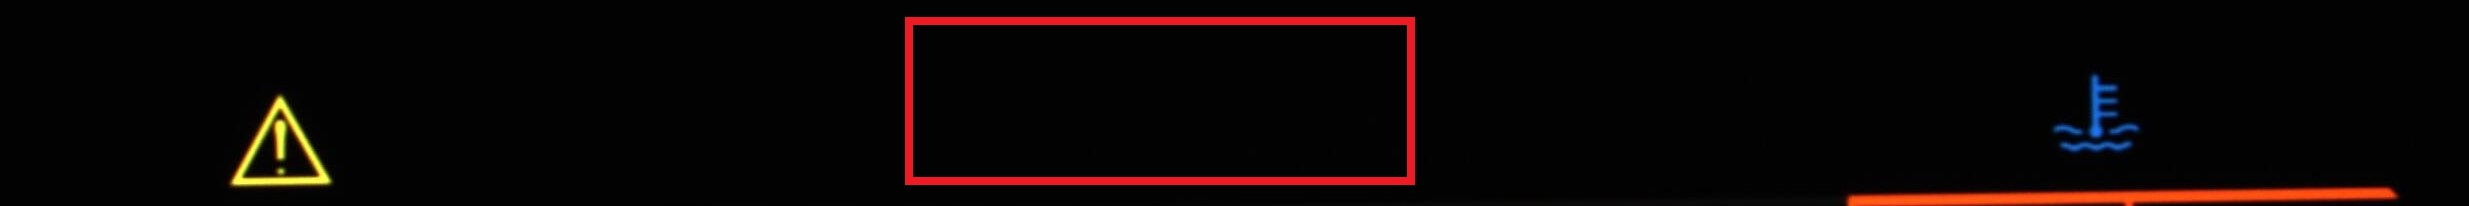
\includegraphics[width=\textwidth]{Figures/GRA_Telltale_OFF_DashboardFailure.jpg}
        \caption{\gls{db} icons actual view}
        \label{fig:IconOutputView}
    \end{subfigure}
    
    \caption{Comparison between \gls{db} icons expected and actual views.}
    \label{fig:CombinedIcons}
\end{figure}

Furthermore, the increased volume of vehicular state information and interactive components on the user interface complicates the task for test engineers, resulting in higher manpower demands and increased costs for the testing process. As a consequence, many \gls{oem}s have resorted to testing only random or high-priority layouts, leaving less critical functionalities out of the test plan. As \gls{sw} complexity continues to grow, ensuring accuracy and comprehensive coverage becomes even more demanding, placing greater strain on testing procedures.

With the introduction of \gls{dl} techniques, these challenges can be effectively addressed by integrating a \gls{cs} with a \gls{hil} setup and an advanced \gls{dl} based \gls{od} algorithm. In this approach, the \gls{hil}  system sends a signal to the \gls{cs} to capture the actual view of the \gls{db}. The \gls{cs} then transmits the captured image back to the \gls{hil}, where the \gls{od} algorithm processes it by extracting all relevant assets and comparing them against reference values to determine whether the displayed view is correct. Further in this chapter, the concepts of testing, \gls{od} techniques and different \gls{cs} that could be used in such a setup will be discussed in details.


\section{Testing}
Testing plays a vital role in the development phase, serving as an evaluation process for systems or applications to detect flaws, mistakes, or glitches, while also confirming that they align with their intended specifications and operate effectively. This practice is crucial because it guarantees that the product functions as specified, meets user requirements and maintains reliability and efficiency \cite{leloudas2023}.

Testing is a continuous process that starts in the early stages of the product development and continues through the product's life cycle. Once the requirements for a product or \gls{sw} are finalized, the testing process can start. The testing process is composed of a well-defined sequence of steps and is known as the \gls{sw} testing life cycle \cite{ML_SW_Testing}. The process consists of planning, designing, executing, and evaluating tests to identify and fix issues, thereby improving the quality of the product \cite{leloudas2023}.

Within the \gls{sw} testing life cycle, various testing methodologies are employed to ensure comprehensive product validation. One of the fundamental approaches is functional testing, which is specifically conducted to verify that the system behaves as expected and meets its defined requirements. Functional testing involves different levels of assessment, each targeting specific aspects of the \gls{sw} functionality. These levels include:

\begin{itemize}
    \item \textbf{Unit testing}: This level of testing involves testing each individual part or module on its own to ensure that it functions correctly.
    \item \textbf{Integration testing}: This level includes testing the integration of all the separate parts together to confirm that they work as a cohesive unit.
    \item \textbf{System testing}: System testing involves testing the entire system as a whole to ensure that it meets all specified requirements.
    \item \textbf{User acceptance testing}: This level looks at the \gls{sw} from the user's perspective to confirm that it performs as they expect and meets their needs.
\end{itemize}

These testing levels are known as the testing pyramid. Figure~\ref{TP} illustrates the test pyramid period, the higher the pyramid level, the higher the integration of the test \cite{leloudas2023}.

\begin{figure}[ht]
    \centering
    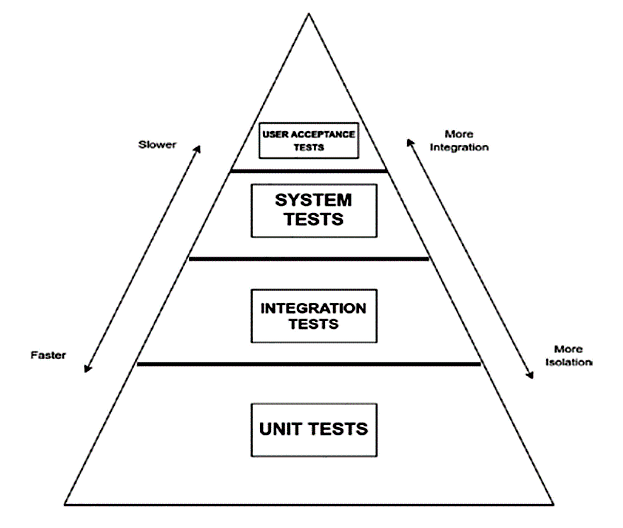
\includegraphics[width=0.7\textwidth]{Figures/Testing_triangle.png}  % Adjust the path and width as needed
    \caption{Testing pyramid consisting of 4 levels: unite tests, integration tests, system tests, user acceptance test \cite{leloudas2023}}
    \label{TP}
\end{figure}

Testing could be defined as a set of steps that are performed in order to validate or evaluate all aspects of a product. It could be done manually in a systematic approach or automated using \gls{sw} scripts \cite{shiwangi2014}. In the following parts of this section, manual and automated testing are explained and compared.


\subsection{Manual Testing}

Manual testing is a process in which test cases are executed by a human tester without the use of automated tools. The tester interacts with the system from an end-user perspective and systematically evaluating its functionalities to identify potential defects, inconsistencies and deviations from expected behavior \cite{shiwangi2014}.
    
Manual testing demands significant investment in human resources and tends to be less reliable, as the precision of tests can fluctuate due to human errors. This approach to testing is slow and significantly time-consuming.


\subsection{Automated Testing}

Automated testing includes specialized \gls{sw} tools used to execute test cases. These tools control the test execution independently of the system being tested. The generated output is then compared to predefined expectations to validate the correct functioning of the system \cite{leloudas2023, shiwangi2014}.

With the growing number of functionalities and interfaces provided by the new generation of \gls{db}, automation offers a solution by executing operations consistently every time the test runs. This approach requires initial investment in the test bench hardware components and scripts development. However, it enhances the testing process efficiency and reduces the possibility of human errors \cite{shiwangi2014}.

\subsection{Manual VS Automated Testing}

The difference between automated and manual \gls{sw} testing lies in their applications and benefits. Table~\ref{tab:comparison automated vs manual testing} provides a summarized comparison of automated and manual testing. It highlights their key differences, unique advantages and applications in \gls{sw} testing. Automated testing is recommended for preventing new errors in previously tested modules. On the other hand, manual testing uses the knowledge of the tester to concentrate on parts of the system thought to be more likely to have problems to excel in identifying new and unforeseen errors. These methods complement each other; automated testing allows for extensive test case coverage in a short period, while manual testing applies human insight to critically assess and target specific, potentially problematic parts of the system \cite{shiwangi2014}. 

\begin{table}[ht]
\centering
\caption{Comparison between Automated and Manual Testing \cite{leloudas2023, shiwangi2014}}
\label{tab:comparison automated vs manual testing}
\begin{tabular}{|p{3cm}|p{6cm}|p{6cm}|}
\hline
\textbf{Aspect} & \textbf{Automated Testing} & \textbf{Manual Testing} \\ \hline
\textbf{Efficiency} & High efficiency due to rapid execution of tests. & Less efficient, as tests are conducted manually. \\ \hline
\textbf{Consistency} & Consistent execution, with the ability to replicate the same test scenarios multiple times. & Potential for inconsistency due to human error. \\ \hline
\textbf{Test Coverage} & Broad test coverage, can run thousands of test cases in one session. & Limited by human capacity, focuses on critical areas rather than extensive coverage. \\ \hline
\textbf{Insight} & Limited to predefined scenarios; lacks human intuition. & Benefits from human insight, allowing for the discovery of unexpected issues. \\ \hline
\textbf{Error Discovery} & Effective in identifying regressions and previously tested functionality errors. & Better at finding new and unforeseen errors through exploratory testing. \\ \hline
\textbf{Focus Areas} & Suited for repetitive, data-driven, and regression tests where consistency is key. & Focuses on high-risk areas and usability testing, relying on the tester's knowledge and experience. \\ \hline
\end{tabular}
\end{table}

\subsection{Testing Requirements}
Testing a component or a system requires some preparation and depends on the type of testing one is planning to perform. In manual testing, the requirements are relatively minimal. For example, testing motor bike \gls{db} as a component requires a handlebar with control buttons , a CAN connector to connect to the pc that simulates the rest of the components communicating with the \gls{db} so that it does not show errors, the \gls{db} itself and a tester. Connecting all these components correctly will result in a component fully functioning and ready to test.

On the other hand, to perform the same tests in an automated approach demands significantly more hardware and \gls{sw} than this. Using the same example of the \gls{db} testing, the basic components required would be:
\begin{itemize}
    \item A \gls{hil} with a real time simulator to control the whole testing process.
    \item  A \gls{cs} acting as the human eye that captures the actual views on the \gls{db}.
    \item Mounting setup with an environment control box to always have the \gls{db} in a controlled and well viewed environment.
    \item An \gls{od} algorithm that will take the images captured by the \gls{cs} to analyze it and extract all the assets with their locations.
    \item Test script that runs on the \gls{hil} to execute a sequence of test cases in an automated way.
\end{itemize}
This setup requires a significant initial investment in terms of time and money, but once it is ready, it will result in the execution of comprehensive component tests multiple times within just a few hours.

Further in this chapter the \gls{od} techniques will be discussed in details, as well as different parameters to consider when choosing a \gls{cs}. This discussion will help in understanding and deciding on the appropriate \gls{cs} and \gls{od} algorithm to use for capturing and analyzing the images, to contribute to the development of a complete automated test setup for \gls{db} testing.


\section{Object Detection}
Recognizing objects in a real-world environment using a machine presents a significant challenge. Computer vision, a specialized field within computer science, provides machines with the capability to perceive, identify, and interpret objects from images and videos. Videos are made up of a series of arranged images, called frames, displayed at a specific rate. While humans can identify objects and their positions within visual data by using their eyes to capture images and transmitting them to the brain for processing, machines rely on \gls{cs} to acquire visual input and employ complex algorithms to process the data and achieve similar capabilities. This technology has been a critical area of research for decades, enabling advancements in applications such as face recognition, pedestrian tracking, security systems, vehicle identification, and autonomous driving \cite{oD_Review}. Recently, \gls{od} has created new opportunities for test engineers to take advantage of these techniques in the field of \gls{db} testing. By integrating \gls{od} methods, engineers can develop more efficient and reliable testing processes, ultimately ensuring the delivery of the highest quality results to the end customer.

\gls{od} is a fundamental process in computer vision, it is defined as the process of integrating object classification and localization to identify and locate multiple objects within an image or video frames. Object classification assigns labels to objects by determining their categories, while object localization identifies their positions. An example of an object classification and localization (\gls{od}) is shown in figure~\ref{Single_object}. In a normal object recognition workflow, an image is analyzed to detect objects, assign labels corresponding to their categories, and calculate the probability for each identified class. Unique object features, such as the equal sides of a square, play a critical role in determining their categories, helping to accurately classify and distinguish between various objects within the image \cite{oD_Review}.

\begin{figure}[ht]
    \centering
    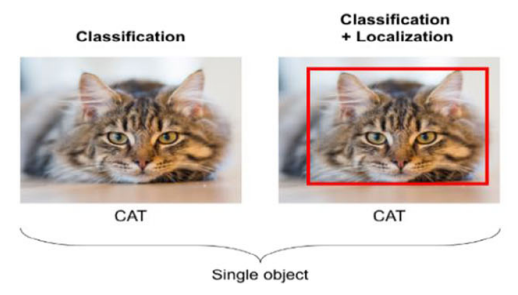
\includegraphics[width=0.7\textwidth]{Figures/Object_detection.PNG} 
    \caption{Single \gls{od} Example \cite{oD_Review}}
    \label{Single_object}
\end{figure}

Choosing the right \gls{od} technique for \gls{db} testing is a vital component of this project to ensure high accuracy and reliable output. The study will explore a range of techniques, including both traditional methods and modern \gls{dl}-based approaches. It will evaluate most popular detection models, analyzing their workflows and identifying their limitations. Additionally, the research will address challenges specific to this domain and investigate potential future advancements to enhance \gls{od} in \gls{db} testing. Figure~\ref{OD_Mindmap} shows how the \gls{od} is divided and structured in this study, which will be further described in details in this section.

\begin{figure}[ht]
    \centering
    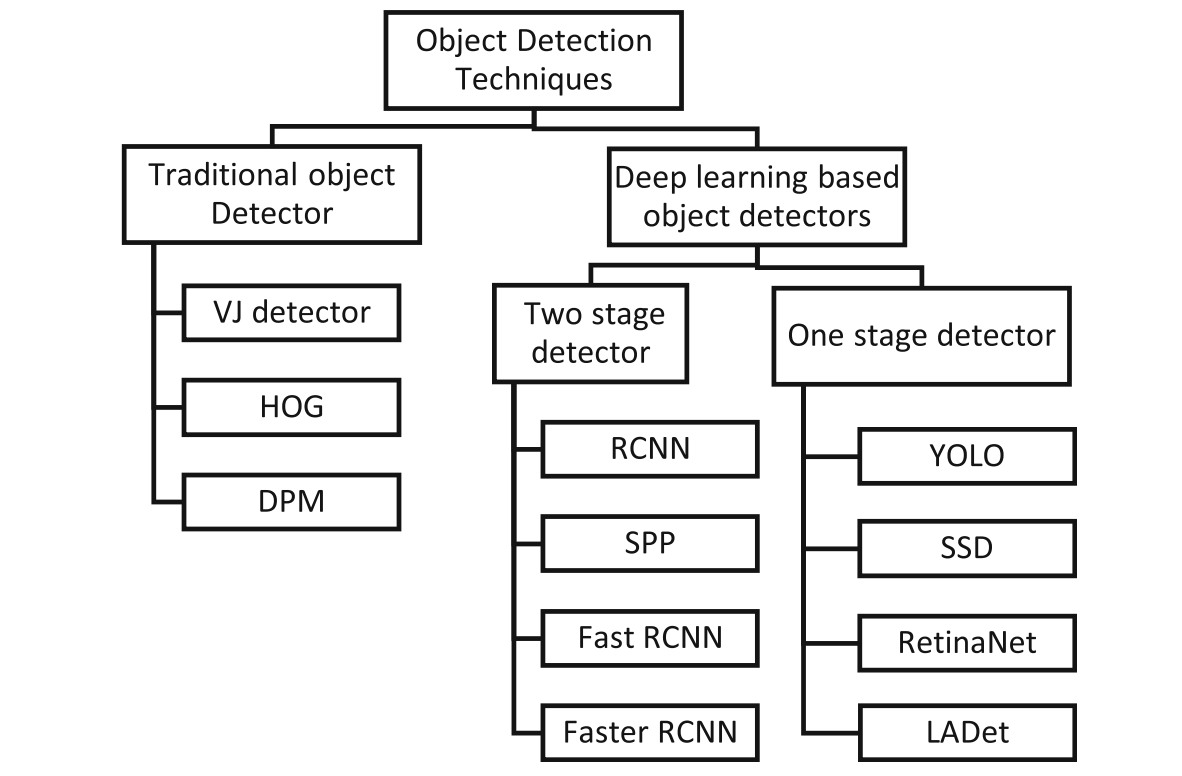
\includegraphics[width=0.7\textwidth]{Figures/OD_Mindmape.PNG} 
    \caption{\gls{od} structure \cite{oD_Review}}
    \label{OD_Mindmap}
\end{figure}

\subsection{Traditional Techniques}
Before modern \gls{ai} and \gls{dl}, traditional \gls{od} methods were used to find objects in images. These methods relied on manually designed features, which are like specific rules or patterns that researchers thought would help identify objects. These features were carefully crafted to focus on important parts of the image, like edges, shapes, or textures. These important parts are known as the \gls{roi}. For example, if one wants to look for a face in a photo, the \gls{roi} might include areas with high contrast like eyes, nose, and mouth, or if one wants to detect a car in an image, the \gls{roi} might focus on the rectangular shapes of windows or wheels.

Over the years, many algorithms were developed. However, the most famous ones are:
\begin{itemize}
    \item \gls{vj} detector which is considered to be the pioneering work that started the development of traditional \gls{od} methods in 2001 \cite{Fam_Traditional_detectors}.
    \item \gls{hog} detector, a feature descriptor which was very popular for \gls{od} and image processing in 2006 \cite{Fam_Traditional_detectors}.
    \item \gls{dpm} with the first introduction of bounding box regression in 2008 \cite{Fam_Traditional_detectors}.
\end{itemize}

A detailed explanation of the three famous detectors will take place in this section. This explanation will help in developing a deeper understanding of the algorithms, their limitations and the current shift to \gls{dl} techniques.

\subsubsection{Viola Jones Detector}
The \gls{vj} detector was named after the authors of this technique “Paul Viola and Michael Jones". It is mainly used for face detection and is considered the first traditional \gls{od} technique. The detection approach is straightforward and efficient, using the sliding window technique to check all the pixels within an image and scale them to help identifying the most important parts of the image like eyes and nose as fast as possible \cite{oD_Review}. Its operation can be divided into four main steps:

\begin{enumerate}
    \item \textbf{Integral Image:}
    The input image is converted into an integral image, to perform efficient calculation of pixel intensity sums over rectangular regions. This reduces the computational cost of feature extraction for any rectangular region.
    
    \item \textbf{Haar-like Features:}  
    Haar-like features are used to represent patterns in the image, such as contrasts between bright and dark regions, such as darker eyes compared to brighter cheeks. These features are calculated by subtracting the sum of pixel intensities in adjacent regions.
    
    \item \textbf{Feature Selection:}  
    Due to the large number of potential Haar-like features, AdaBoost is used to select the most relevant characteristics. AdaBoost combines many weak classifiers into a strong classifier. It assigns higher weights to features that distinguish between faces and non-faces betters.

    \item \textbf{Detection Cascade:}  
    The last step of the \gls{vj} detector is a cascade of classifiers. It is used to discard the background region from the image and focuses the computational power on the objects itself rather than the complete image. It consists of multiple stages where each stage filters out non-face regions. The early stages use simple classifiers to eliminate most of the image, while the later stages apply a more complex analysis to regions likely to contain faces.

\end{enumerate}

While the \gls{vj} detector was a groundbreaking approach for \gls{od} it had some limitations had limitations in handling complex variations in object appearance. To overcome some of these challenges, the \gls{hog} detector was introduced.

\subsubsection{Histogram Of Oriented Gradients}
 \gls{hog} is one of the most famous feature descriptors. Feature descriptors are methods that transform raw data into a more simplified form that contains only the most important features to minimize the required computational power. \gls{hog} describes the shape and appearance of the object by analyzing the distribution of edge orientations. The \gls{hog} method calculates the gradient magnitude and orientation for each pixel in an image and partitions the image into small cells, unlike simple edge features that only detect edges without direction. The image is divided into smaller regions (localized portions), and gradients and orientations are computed for each region. A histogram is then generated for each region based on these gradients and orientations \cite{HOG}. Figure~\ref{HOG_image} shows the comparison between the input image and the \gls{hog} image.
 
\begin{figure}[ht]
    \centering
    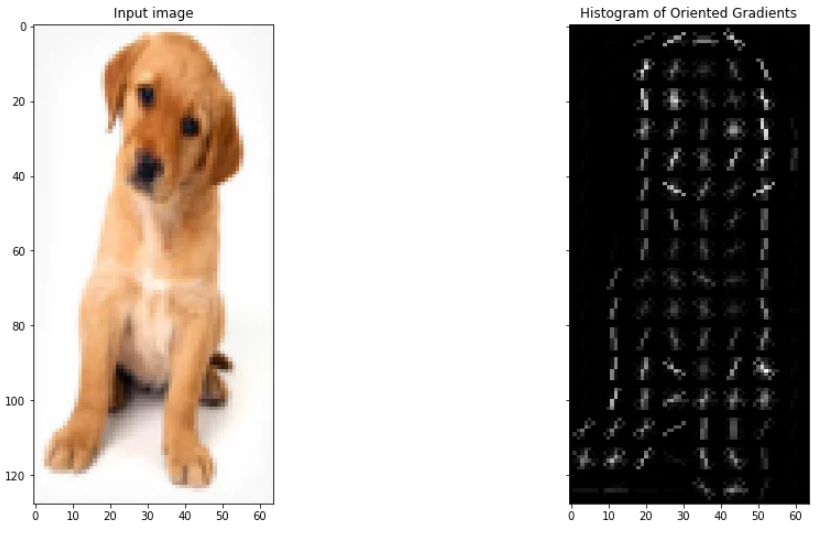
\includegraphics[width=0.7\textwidth]{Figures/HOG_Histogram_image.PNG} 
    \caption{Input image and \gls{hog} image \cite{HOG}}
    \label{HOG_image}
\end{figure}

The extracted information is then passed to \gls{ml} algorithms, such as \gls{svm}, to train the classifier. To eliminate redundant bounding boxes, \gls{nms} is applied. \gls{hog} is used for detecting objects across various classes and sizes by repeatedly re-scaling the image while maintaining a fixed window size. It has been widely applied, particularly in pedestrian detection \cite{oD_Review}.

Although \gls{hog} detectors improved the robustness of the detection over \gls{vj}, they still lacked the flexibility to represent variation in objects. This limitation opened the door for \gls{dpm} development to help overcome this limitation.

\subsubsection{Deformable Part-Based Models}
\gls{dpm} represent a significant leap forward in traditional \gls{od} methods. By building on the foundation of HOG detectors, \gls{dpm} introduces a "divide-and-conquer" strategy. During the training or "divide" phase, the model learns how to break down objects into smaller, easily recognizable components. In the inference or "conquer" phase, these components are reassembled to predict the complete object \cite{oD_Review}.

The \gls{dpm} framework is composed of three primary components: the root filter, part filters, and a spatial model. The root filter acts as the detection window, roughly outlining the entire object by applying a weighted filter to a feature vector extracted from the selected region. Meanwhile, the part filters focus on identifying smaller parts of the object, allowing the model to achieve a more detailed analysis. The spatial model then assesses the relative arrangement of the part filters in relation to the root filter. By scoring the placement of these parts, it enhances the precision of \gls{od}. This breakdown and integration of object parts make \gls{dpm} a foundational tool in \gls{od} techniques \cite{oD_Review}.

\subsubsection{Limitations}
In conclusion, most of traditional \gls{ml} \gls{od} techniques depend on scanning the image and identifying the potential regions of interest that might contain the object. After that it extracts its characteristics such as \gls{hog} and other information that might be relevant. It then uses a distinct classifier to identify different types of items and determine whether objects are present within the specific subregion. This process comes with some limitations, such as the difficulty in training the classifier and feature extractor, the high computational demand, high development effort for manual feature extraction, and the failure to accurately identify the position of objects \cite{OD_Survey}. Rapidly it was realized that a more sophisticated, reliable and accurate approach is needed to fulfill the requirements of different industries.


\subsection{The Shift To Deep Learning}
The field of \gls{od} has seen a significant transformation, transitioning from traditional \gls{ml} methods to state-of-the-art \gls{dl} approaches. Unlike traditional methods that rely on hand-crafted features, modern \gls{dl}-based techniques automatically learn intricate and hierarchical representations directly from the data. This capability enables more accurate, adaptable, and scalable detection systems.  

\gls{dl}-based detectors excel at recognizing complex patterns and finding variations within images, significantly outperforming conventional approaches, particularly in challenging tasks such as image classification and \gls{od}. By using the multi-layered feature extraction capabilities of \gls{dnn}, these systems can effectively address diverse scenarios, including variations in lighting conditions, occlusions, and object scales. This shift marks a transformative advancement in \gls{od}, providing robust and precise solutions for different industries, from autonomous vehicles to medical imaging and security systems.  

What is \gls{dl}, and How is it different from \gls{ml}? 

Both \gls{dl} and \gls{ml} are branches of \gls{ai}, but they differ in scope and methodology. \gls{ml} is a broader concept that contains a variety of algorithms capable of learning from data, including simpler techniques such as decision trees, \gls{svm}s, and ensemble models. In contrast, \gls{dl} is a specialized subset of \gls{ml} that uses an artificial \gls{nn}, inspired by the structure and functioning of the human brain to process and learn complex patterns from data  \cite{DL_VS_ML} \cite{oD_Review}.

While both \gls{ml} and \gls{dl} can be trained on labeled or unlabeled data, \gls{dl} has an advantage when solving tasks that involve complex pattern recognition. Examples include image recognition, speech recognition, and natural language processing, where \gls{dl} often outperforms traditional \gls{ml} by automatically learning multi-level features without human intervention  \cite{DL_VS_ML} \cite{oD_Review}.  

At the core of \gls{dl} are artificial \gls{nn}s, consisting of interconnected node layers (neurons). These networks typically include an input layer, one or more hidden layers, and an output layer. Each neuron is connected to others through weighted connections and has an associated threshold. When a neuron's output exceeds its threshold, it becomes activated, passing data to the next layer; otherwise, no information is transmitted \cite{ibm_cnn}. During the training process, the weights between these nodes are iteratively adjusted to minimize errors and improve performance using the activation functions. This optimization process can be achieved using approaches such as supervised learning, unsupervised learning, or reinforcement learning depending on the problem at hand  \cite{DL_VS_ML} \cite{oD_Review}. Figure~\ref{DNN} shows a schematic of a \gls{dnn}. 

\begin{figure}[ht]
    \centering
    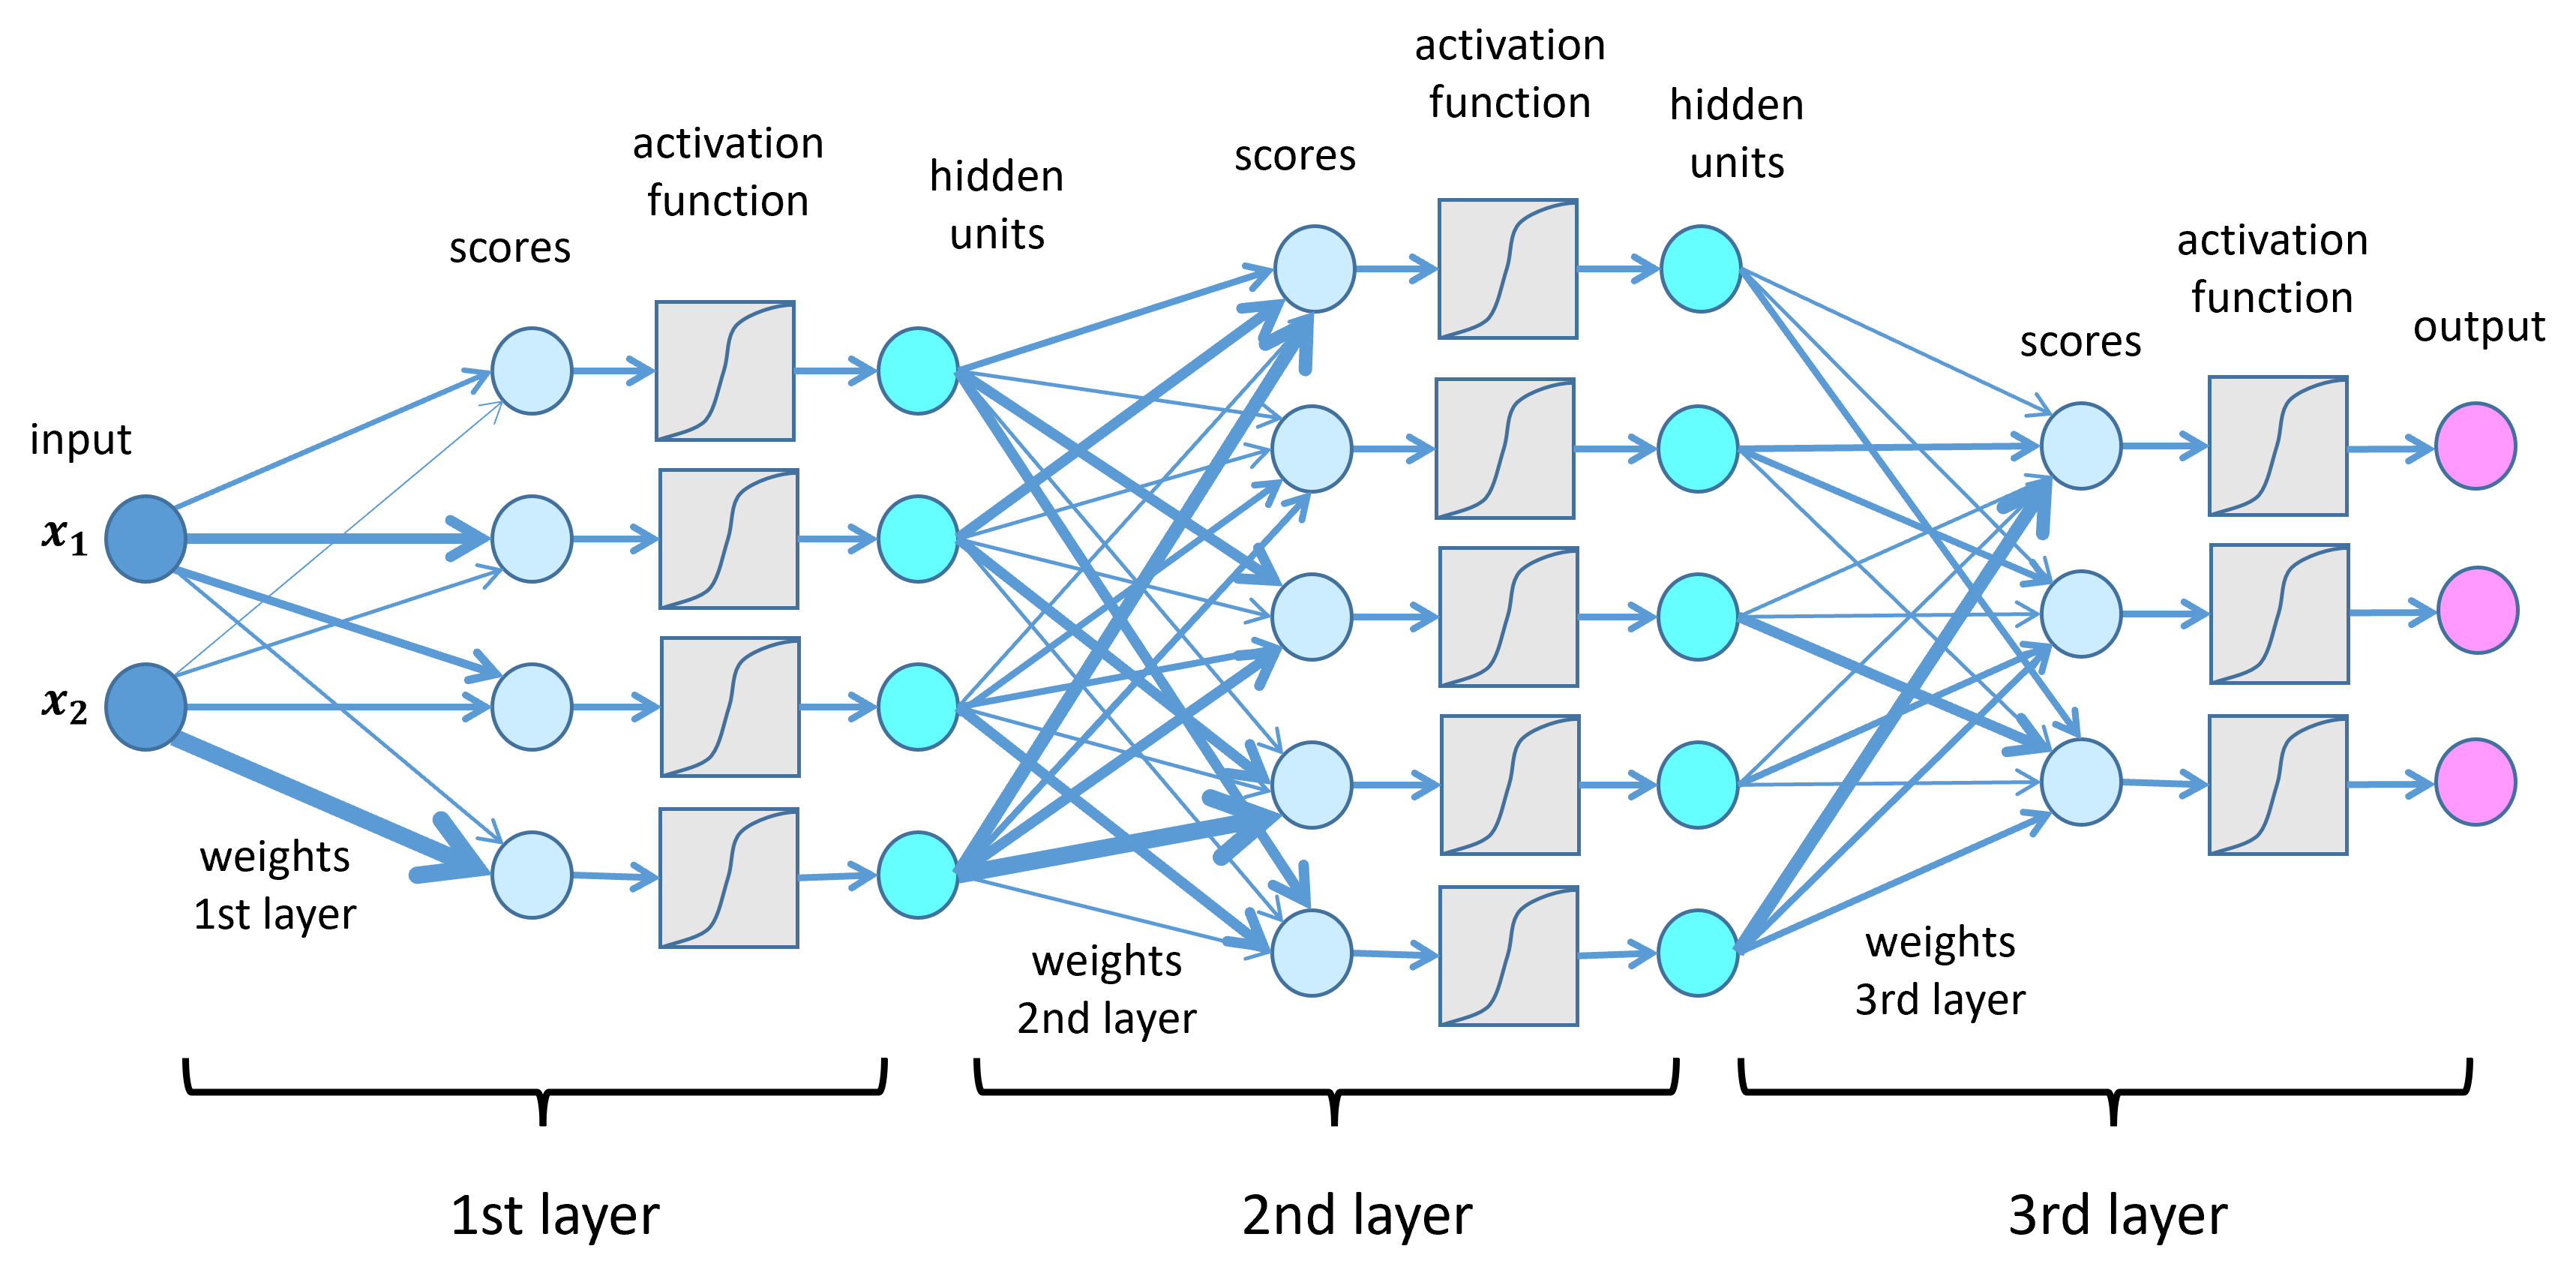
\includegraphics[width=0.9\textwidth]{Figures/deepLearn_2_EN.png} 
    \caption{A \gls{dnn} with multiple layers, illustrating the flow of data from input to output through interconnected hidden layers \cite{DNN_pic}.}
    \label{DNN}
\end{figure}

Once trained, a \gls{nn} can efficiently analyze new unseen data and make highly accurate predictions, making it an invaluable tool for solving complex real-world problems. The ability of \gls{dl} to adapt to large unstructured data sets and uncover hidden relationships within them has strengthened its role as a revolutionary advancement in \gls{ai} \cite{DL_VS_ML} \cite{oD_Review}.

The \gls{nn}s mentioned above are the simplest form of \gls{nn}s and are known as feedforward \gls{nn}s. However, there are different types of \gls{nn}s nowadays, focusing on different tasks and data types. For example,  in natural language processing and speech recognition, one can use recurrent \gls{nn}s. On the other hand, when dealing with a classification problem or a computer vision task, one can depend on \gls{cnn}s. \gls{cnn}s offer a scalable solution for image classification and object recognition by utilizing concepts from linear algebra like matrix multiplication to detect patterns within images \cite{ibm_cnn}.

\subsection{Convolutional Neural Networks}
\gls{cnn}s often consists of 3 main types of layers, \gls{cl}, \gls{pl} and \gls{fcl}. The first layer is always the \gls{cl}, it could be then followed by another \gls{cl} or a \gls{pl} and the final layer is always an \gls{fcl}. Figure~\ref{full_cnn} shows a schematic of a \gls{cnn} architecture. As a \gls{cnn} processes an image through these multiple layers, it gradually builds a more detailed understanding of the content of the image. The initial layers detect basic features like edges and colors, while deeper layers analyze more complex patterns and structures. As the data moves through the network, it begins to recognize larger shapes and meaningful components, ultimately leading to the identification of the entire object.

\begin{figure}[ht]
    \centering
    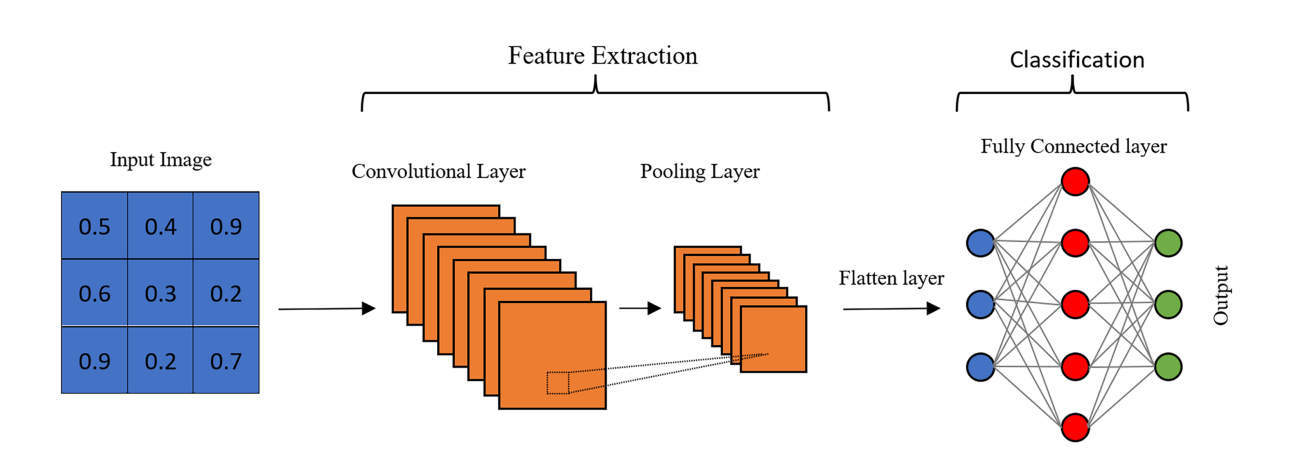
\includegraphics[width=0.9\textwidth]{Figures/Full_cnn.PNG} 
    \caption{\gls{cnn} architecture \cite{Full_CNN}.}
    \label{full_cnn}
\end{figure}

\subsubsection{Convolutional Layer}
The \gls{cl} is the fundamental component of a CNN, where most computations occur. It operates using three key elements: input data, filters (kernels), and feature maps. An RGB image, represented as a three dimensional matrix of pixels (height, width, and depth for RGB channels), is processed by moving a small filter across it in a process called convolution. The filter, typically a 3×3 matrix, slides over the image, computing a dot product between its weights and the pixel values, generating an activation map (feature map). Figure~\ref{cnn_cl} explains the full process that happens within the \gls{cl}. This process is controlled by three hyperparameters:
\begin{itemize}
    \item The \textbf{number of filters}, which determines the depth of the output. Three distinct filters would result in three different feature maps, creating a depth of three \cite{ibm_cnn}.
    \item The \textbf{stride}, which defines the step size of the filter's movement. The larger the stride, the smaller the output \cite{ibm_cnn}.
    \item \textbf{zero padding}, which manages the image borders to maintain size consistency. Padding can also be \textbf{valid padding} (no padding), \textbf{same padding} (output size matches input), or \textbf{full padding} (expands the image with zeros) \cite{ibm_cnn}.
\end{itemize}   
After convolution, a Rectified Linear Unit (ReLU) function is applied to introduce non-linearity, helping the model learn complex patterns efficiently \cite{ibm_cnn}.

\begin{figure}[ht]
    \centering
    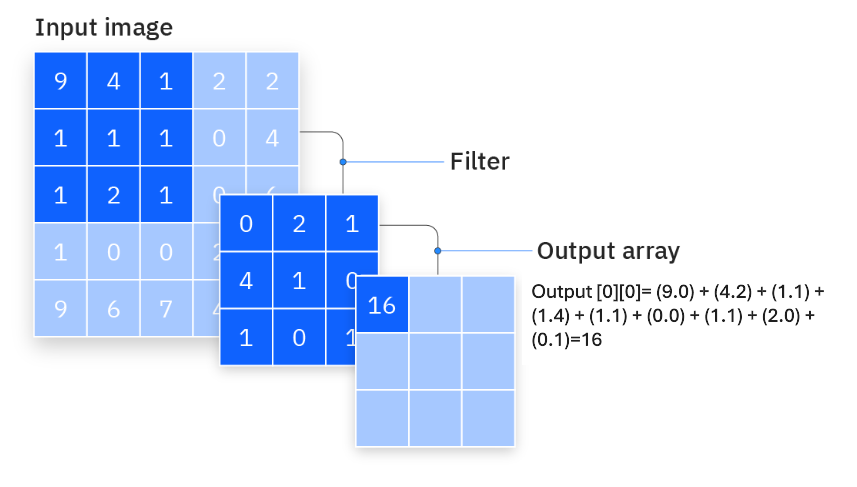
\includegraphics[width=0.9\textwidth]{Figures/CNN_CL.PNG} 
    \caption{Convolutional process and dot product calculation of an input image \cite{ibm_cnn}.}
    \label{cnn_cl}
\end{figure}

As mentioned earlier, a \gls{cl} could be followed by another \gls{cl}. This setup forms a hierarchical structure where later layers analyze patterns identified by earlier ones. This is normally used in more complex tasks because it allows the network to break down the object into lower level features and then assemble these feature into one higher level representation \cite{ibm_cnn}.

\subsubsection{Pooling Layer}
The \gls{pl} benefits \gls{cnn}s by lowering computational complexity, improving efficiency, reducing the risk of overfitting and helping the model generalize better to new data. It reduces the dimensionality of the data by reducing the number of parameters in the input. \gls{pl} uses a sliding filter across the input, but unlike convolution, the filter does not contain weights. Instead, it applies an aggregation function to the values within its receptive field to generate a simplified output representation \cite{ibm_cnn}. There are two main \gls{pl} types:

\begin{itemize}
    \item \textbf{Max pooling:} The filter selects the highest pixel value within its receptive field and passes it to the output \cite{ibm_cnn}.
     \item \textbf{Average pooling:} The filter computes the average value of the pixels in its receptive field and sends this to the output \cite{ibm_cnn}.
\end{itemize}

In general the max pooling is more preferred over the average pooling because it helps retain essential features. The \gls{pl} comes with a downside which is loss of information. However, the benefits is much higher which makes it valuable in \gls{cnn} \cite{ibm_cnn}.

\subsubsection{Fully Connected Layer}
The \gls{fcl} layer gets its name from its structure, where each neuron is directly linked to every neuron in the previous layer. This layer is responsible for the classification task. \gls{fcl} uses the features extracted from the previous \gls{cl} and \gls{pl} and a softmax function, which assigns probabilities to different classes to help the model determine the most likely category for the input \cite{ibm_cnn}.



\subsection{Deep Learning Techniques For Object Detection}
DL-based \gls{od} techniques are categorized into two-stage and one-stage detectors. Two-stage detectors detect objects in two steps, often achieving state-of-the-art accuracy on benchmark datasets, but at the cost of slower inference speeds. In contrast, one-stage detectors are primarily used for real-time \gls{od}, offering faster results while maintaining satisfactory accuracy \cite{oD_Review}.

\subsubsection{Two Stage Detectors}
Two-stage detectors, also known as multi-stage detectors, typically comprise two models. The first model identifies the \gls{roi}, while the second model classifies objects and refines their localization. These detectors are renowned for delivering state-of-the-art performance in \gls{od}, but this comes at the cost of slower processing speeds and high computational demands \cite{oD_Review}.

\begin{enumerate}
    \item \textbf{\gls{rcnn}:} \gls{rcnn} is a two-stage object detector that operates in three steps: region extraction, \gls{cnn} feature computation, and region classification with localization. In the region extraction step, a selective search algorithm generates approximately 2000 candidate regions by grouping similar regions based on size, texture, color, and shape. Each region is then resized to a fixed size and passed through a \gls{cnn} to extract features. Finally, in the region classification step, an \gls{svm} classifier assigns scores to each class, and \gls{nms} is applied to eliminate overlapping regions whose intersection over union exceeds a predefined threshold \cite{oD_Review}. Figure~\ref{RCNN} shows a schematic describing the basic steps for \gls{rcnn} to detect a dog in a picture.

    This approach not only classifies objects but also provides bounding boxes around detected objects. However, \gls{rcnn}s come with some limitations. Features are extracted from each proposal separately using a deep \gls{cnn}, leading to redundant computations and making the training and testing processes time-consuming. Additionally, the three steps of this method are independent and operate separately, which makes it challenging to achieve a globally optimal solution. Lastly, in images with complex backgrounds, the selective search algorithm struggles to generate effective proposals because it relies solely on low-level features \cite{oD_Review}.
    
    \begin{figure}[ht]
        \centering
        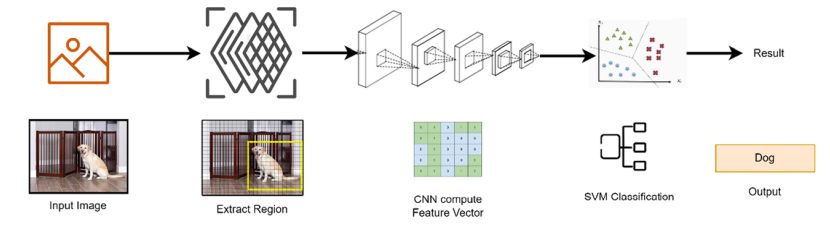
\includegraphics[width=0.9\textwidth]{Figures/RCNN.PNG} 
        \caption{Steps involved in \gls{rcnn} detector \cite{oD_Review}.}
        \label{RCNN}
    \end{figure}
    
    \item \textbf{\gls{spp-net}:} A new network was introduced in 2014 to overcome the limitations of the \gls{rcnn} called \gls{spp-net}. In \gls{rcnn}, the input image is resized to a fixed size before being processed by the \gls{cnn}, which can crop or distort objects, thereby reducing accuracy. \gls{spp-net} solves this problem by removing the fixed size requirement and using a SPP layer to improve accuracy. \gls{spp-net} processes the entire image at once to create a feature map, then divides this feature map into fixed-size grids at multiple scales as shown in figure~\ref{SPP}. From each grid cell, a fixed-length feature vector is created. These feature vectors are combined and passed to soft vector machine classifiers and a bounding box regressor to detect and localize objects. 
    
    \gls{spp-net} achieves accuracy comparable to \gls{rcnn} while being 20 times faster. However, it has its downsides. One key limitation is that it does not take full advantage of the \gls{cnn}. Another drawback lies in its multi-stage training process, which can complicate implementation. Despite these limitations, \gls{spp-net} excels at handling images with different scales and aspect ratios. It effectively preserves image details and avoids distortions that might otherwise compromise the performance of the model \cite{oD_Review}.

    \begin{figure}[ht]
        \centering
        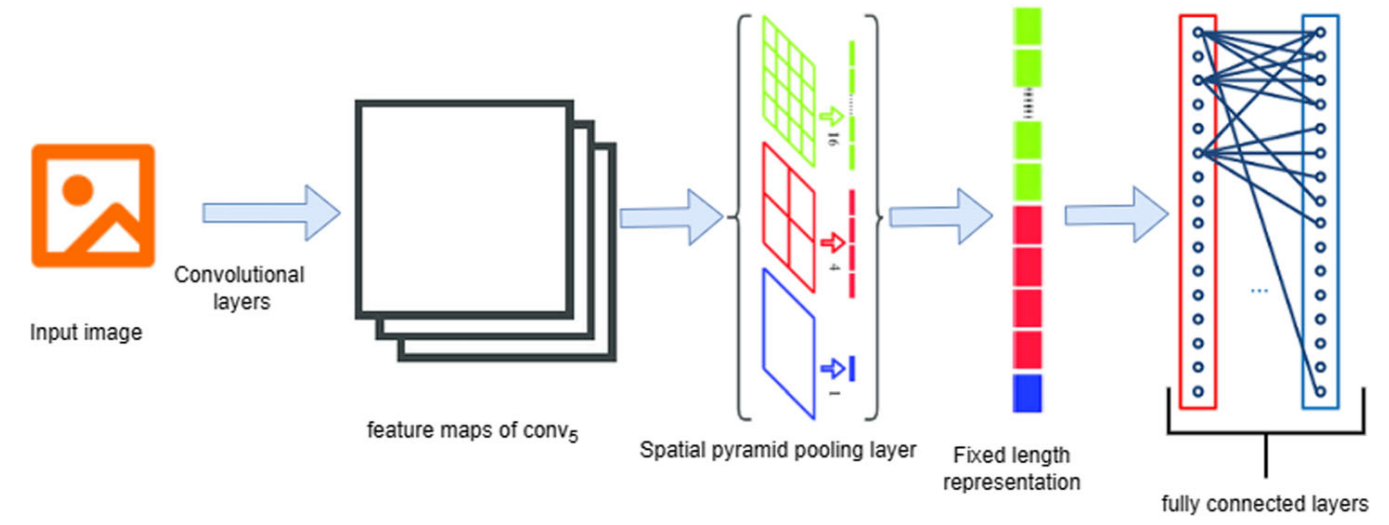
\includegraphics[width=0.9\textwidth]{Figures/SPP.PNG} 
        \caption{Steps involved in \gls{spp-net} detector \cite{oD_Review}.}
        \label{SPP}
    \end{figure}

    
    \item \textbf{Fast \gls{rcnn}:} Further improvements were made to \gls{rcnn} and SPPNet and a new architecture was introduced called Fast \gls{rcnn}. Fast \gls{rcnn} processes the entire input image to produce feature maps using a convolutional layer. It simplifies the design by removing multi-level pooling layers and instead uses a single grid layer. A \gls{roi} pooling layer is introduced to extract a fixed length feature vector, that acts as a simplified version of the SPP layer with just one pyramid level \cite{oD_Review}.

    Each feature vector is processed through a sequence of \gls{fcl}, and the final output is fed into two layers: the softmax layer and the bounding box regression layer. The softmax layer calculates probabilities for all object classes and a background class, while the bounding box regression layer generates four real values to define the bounding box for each detected object. Figure~\ref{Fast_RCNN} shows the architecture used to developed a Fast \gls{rcnn} \cite{oD_Review}.
    \begin{figure}[ht]
        \centering
        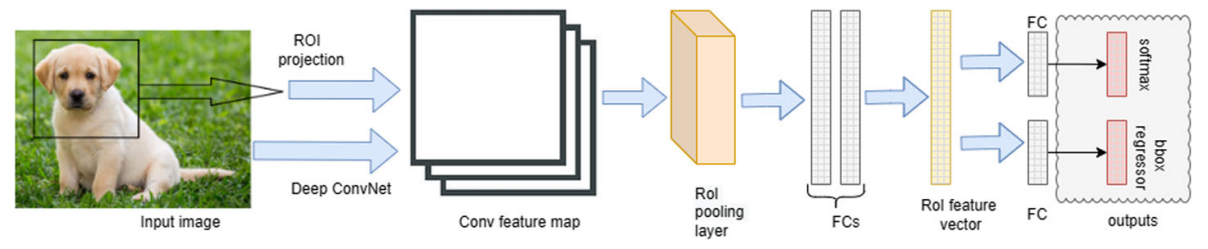
\includegraphics[width=0.9\textwidth]{Figures/Fast-RCNN.PNG} 
        \caption{Fast \gls{rcnn} architecture \cite{oD_Review}.}
        \label{Fast_RCNN}
    \end{figure}

    Fast \gls{rcnn} eliminates the need for separate training for classification and bounding box regression. It was implemented using Python and C++. This method combines the strengths of \gls{rcnn} and \gls{spp-net}, offering improved accuracy and efficiency. However, it is slightly slower due to the proposal detection process. Despite this, it reduces storage requirements and enhances overall performance \cite{oD_Review}.


    \item \textbf{Faster \gls{rcnn}:} In 2015, a new method called Region Proposal Network (RPN) was introduced to improve the performance of Fast \gls{rcnn}. RPN replaces traditional region generation methods like selective search and edge boxes. It uses a sliding window approach on the feature map to generate bounding boxes for objects, each with a confidence score. These bounding boxes, referred to as anchor boxes, are designed with a common aspect ratio. Once the proposals are generated, they are resized to a fixed size and passed through the \gls{fcl}, followed by a softmax layer and a regression layer for classification and bounding box refinement. To increase non-linearity, a ReLU activation function is applied to the output of the convolution window. This new architecture enables end-to-end training of the \gls{od} algorithm, making the process more efficient \cite{oD_Review}.
\end{enumerate}

\subsubsection{One Stage Detector}
The idea of the one stage detectors is to remove the intermediate task to take the final output. Hence, increasing the speed of the detection and reducing the computational demand while maintaining high accuracy. The one stage detectors are very useful in real time detection applications that require high speed detection like autonomous systems.

\begin{enumerate}
    \item \textbf{\gls{yolo}:} In 2015, \gls{yolo} was introduced as the first single-stage \gls{od} framework. It uses a deep \gls{cnn} to process the entire input image and detect objects. The initial 20 convolutional layers are pre-trained on the ImageNet dataset, with modifications made for \gls{od} tasks. \gls{yolo}’s \gls{fcl} predicts both class probabilities and bounding box coordinates.

    \gls{yolo} divides the image into an S × S grid, assigning each grid cell the responsibility of detecting objects whose centers fall within it. Each cell predicts bounding boxes with confidence scores, indicating the likelihood of containing an object and the accuracy of the box.

    To improve efficiency, \gls{yolo} assigns one bounding box predictor per object based on the highest intersection over union with the ground truth. This specialization enhances recall by focusing on specific object sizes, shapes, and classes. \gls{nms} is then applied as a post-processing step to eliminate redundant bounding boxes, ensuring that only one box is retained per object \cite{YOLO}. Figure~\ref{YOLO} explains the architecture of \gls{yolo}. \gls{yolo} kept on developing over the years and many versions are published until \gls{yolo}v11. Table~\ref{tab:yolo_versions} summarizes all \gls{yolo} versions and their key improvments

    \begin{figure}[ht]
        \centering
        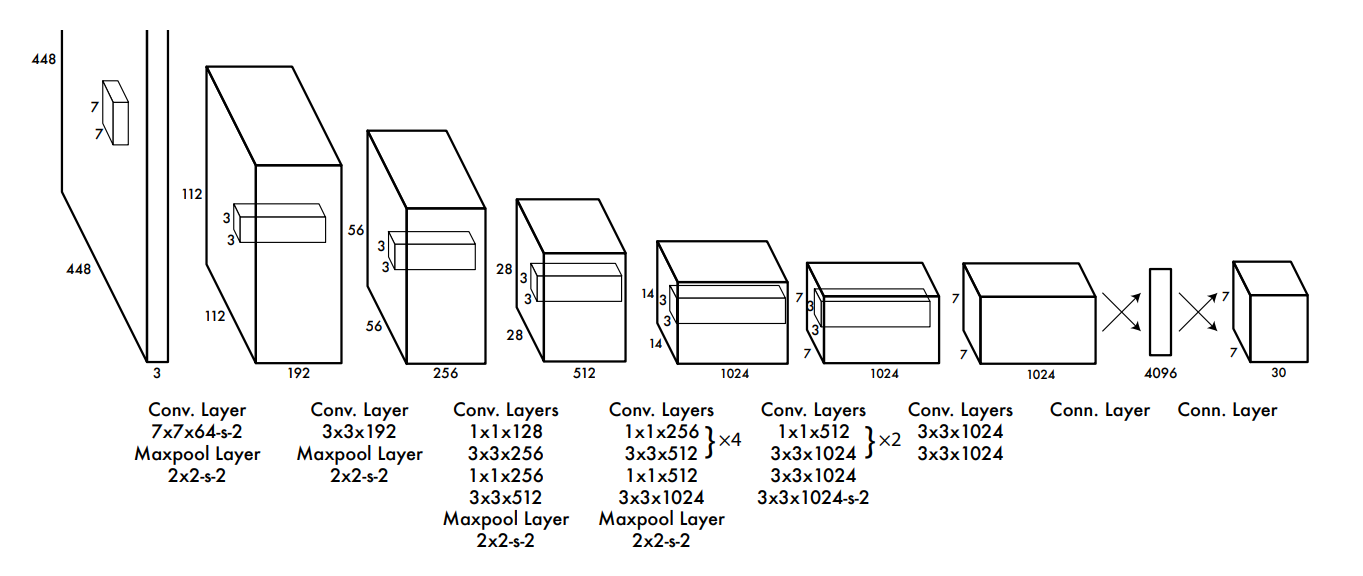
\includegraphics[width=0.9\textwidth]{Figures/YOLO.PNG} 
        \caption{\gls{yolo} Architecture that consists of 24 convolutional layers followed by 2 \gls{fcl}s \cite{YOLO}.}
        \label{YOLO}
    \end{figure}


    \begin{table}[h!]
    \centering
    \begin{tabular}{|c|p{12cm}|}
    \hline
    \textbf{Version} & \textbf{Key Features and Improvements} \\
    \hline
    \gls{yolo}v2 (2016) & Added batch normalization, anchor boxes, and dimension clusters to improve the original model. \\
    \hline
    \gls{yolo}v3 (2018) & Introduced a more efficient backbone network, multiple anchors, and SPP for enhanced performance. \\
    \hline
    \gls{yolo}v4 (2020) & Featured mosaic data augmentation, a new anchor-free detection head, and a new loss function. \\
    \hline
    \gls{yolo}v5 & Included hyperparameter optimization, experiment tracking, and automatic export to popular formats for better performance. \\
    \hline
    \gls{yolo}v6 (2022) & Open-sourced by Meituan and used in autonomous delivery robots. \\
    \hline
    \gls{yolo}v7 & Added pose estimation capabilities, including support for the COCO keypoints dataset. \\
    \hline
    \gls{yolo}v8 (2023) & Released by Ultralytics with improved performance, flexibility, and efficiency, supporting various vision \gls{ai} tasks. \\
    \hline
    \gls{yolo}v9 & Introduced Programmable Gradient Information (PGI) and the Generalized Efficient Layer Aggregation Network (GELAN). \\
    \hline
    \gls{yolo}v10 & Developed by Tsinghua University, featuring an End-to-End head that eliminates the need for \gls{nms}. \\
    \hline
    \gls{yolo}v11 & The latest version by Ultralytics, delivering state-of-the-art performance across multiple tasks like detection, segmentation, pose estimation, tracking, and classification. \\
    \hline
    \end{tabular}
    \caption{Summary of \gls{yolo} Versions and Their Key Features \cite{ultralytics_yolo_history}}
    \label{tab:yolo_versions}
    \end{table}

    \item \textbf{\gls{ssd}:} The \gls{ssd} was introduced in November 2016 and marked a significant milestone in \gls{od} by achieving over 74\% \gls{map} at 59 \gls{fps} on standard datasets like PascalVOC and COCO as shown in figure~\ref{SSD}. The name of the architecture reflects its key principles: "Single Shot" indicates that object localization and classification are performed in a single forward pass through the network, while "MultiBox" refers to a bounding box regression technique developed by Szegedy et al. The "Detector" aspect highlights its capability to both detect and classify objects simultaneously \cite{SSD}.

    \gls{ssd} is built on the VGG-16 architecture but discards the \gls{fcl}s in favor of auxiliary convolutional layers starting from conv6. This design enables the model to extract features at multiple scales while progressively reducing the input size for each subsequent layer. VGG-16 was selected as the base network due to its strong performance in high-quality image classification tasks and its effectiveness in improving results through transfer learning \cite{SSD}.

    \begin{figure}[ht]
        \centering
        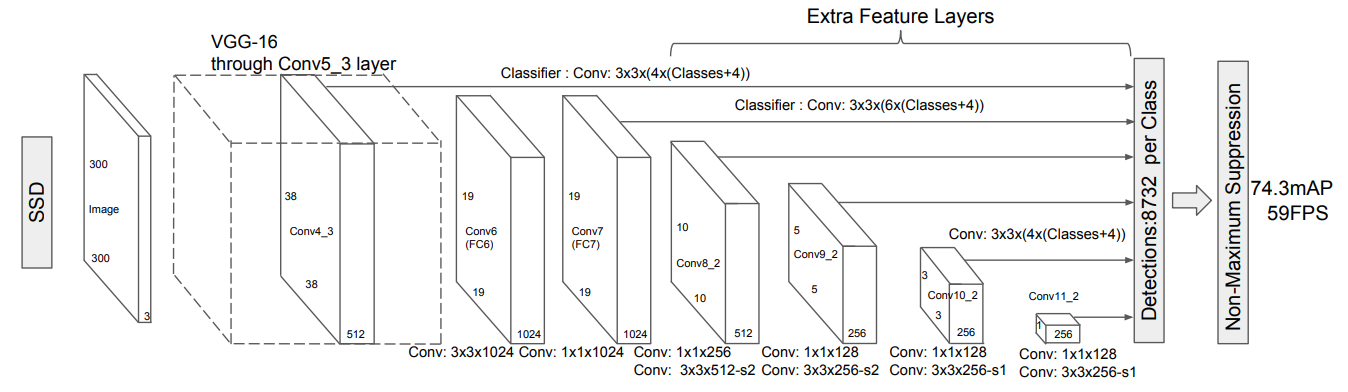
\includegraphics[width=0.9\textwidth]{Figures/SSD.PNG} 
        \caption{\gls{ssd} Architecture that is based on VGG-16 for \gls{od} with 59 \gls{fps} \cite{SSD}.}
        \label{SSD}
    \end{figure}

    \item \textbf{RetinaNet:} RatinaNet is a one-stage \gls{od} framework designed to address class imbalance during training through an innovative loss function known as focal loss. This loss function introduces a modulating factor to the standard cross-entropy loss, It focuses more on difficult examples while giving less attention to those that are already easy to classify. The RetinaNet model integrates two main components: a backbone network and two task-specific subnetworks. The backbone, typically a pre-trained \gls{cnn}, generates a feature map from the input image. On top of this backbone, one subnetwork handles object classification, while the other focuses on bounding box regression \cite{RatinaNet}. 

    A key advantage of RetinaNet lies in its ability to handle class imbalance without relying on the cascaded sampling techniques commonly used in two-stage detectors. In traditional two-stage detectors, the proposal stage filters out most background samples, then the classification stage uses heuristics like fixed foreground-to-background ratios or online hard example mining. On the other hand, RetinaNet processes a larger set of candidate locations uniformly sampled across the image. It uses focal loss to dynamically scale the cross-entropy loss in a way that reduces its influence for well-predicted classes, allowing the model to focus on challenging cases \cite{RatinaNet}.

    The network architecture is shown in figure~\ref{Ratina} and includes four components: a bottom-up pathway using a ResNet backbone, a top-down pathway enhanced with feature pyramid networks, a classification subnetwork, and a regression subnetwork. The feature pyramid networks allows effective feature extraction across multiple scales, facilitating the detection of objects of varying sizes. The classification subnetwork predicts the probabilities of the object class and the anchor boxes, while the regression subnetwork refines the offsets of the bounding box. This multi-scale capability makes RetinaNet particularly effective for detecting small or densely packed objects \cite{oD_Review}.

     \begin{figure}[ht]
        \centering
        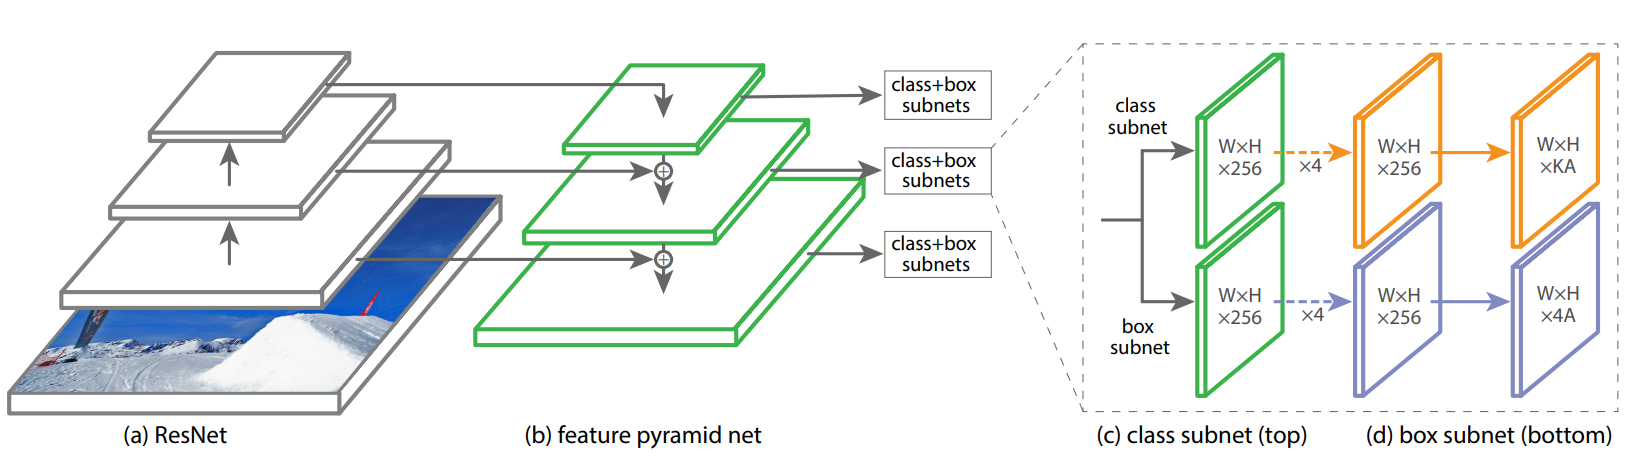
\includegraphics[width=0.9\textwidth]{Figures/ratina-net.PNG} 
        \caption{RetinaNet architecture: (a) ResNet backbone generates multi-scale feature maps, (b) Feature Pyramid Network enhances multi-scale feature extraction, (c) classification subnetwork predicts class probabilities, and (d) box subnetwork refines anchor boxes to ground-truth object boxes \cite{oD_Review}.}
        \label{Ratina}
    \end{figure}

    RetinaNet’s performance equals that of two-stage detectors in terms of high detection accuracy while outperforming it in fast detection speeds. Its capabilities have been demonstrated in multiple applications, including aerial and satellite imagery analysis. Furthermore, advanced variations like R4 (Refined Single-Stage Detector with Feature Recursion and Refinement) have extended its capabilities for handling complex challenges such as dense object distributions, large aspect ratios, and category imbalances \cite{oD_Review}.

     \item \textbf{LADet:} LADet is a lightweight and adaptive network designed for multi-scale \gls{od}. LADet addresses challenges in \gls{od} like variations in object size through two innovative components: the \gls{afpm} and the \gls{lcfm}. \gls{afpm} improves the integration of semantic information across different feature map levels, moving away from traditional top-down structures. \gls{lcfm} optimizes anchor box usage with minimal computational overhead, using sparse convolution techniques for better efficiency. Together, these components improve detection accuracy while maintaining computational efficiency \cite{LADet}.

     The structure of LADet begins with a backbone network (e.g., DenseNet-169 or VGG-16) extracting multi-level feature maps. These maps are processed through the \gls{afpm}, which includes the Feature Fusion Module. Feature Fusion Module normalizes feature maps to a uniform resolution and fuses them into a unified high-resolution representation. This fusion ensures effective contribution from all scales. Complementary semantic information is added via a channel-wise attention mechanism, refining feature maps further for precise detection. The \gls{lcfm} then predicts object classes and anchor box probabilities using sparse group convolutions, reducing parameter usage while maintaining performance \cite{LADet}. Figure~\ref{LADet} shows an overview of the network structure.

     \begin{figure}[ht]
        \centering
        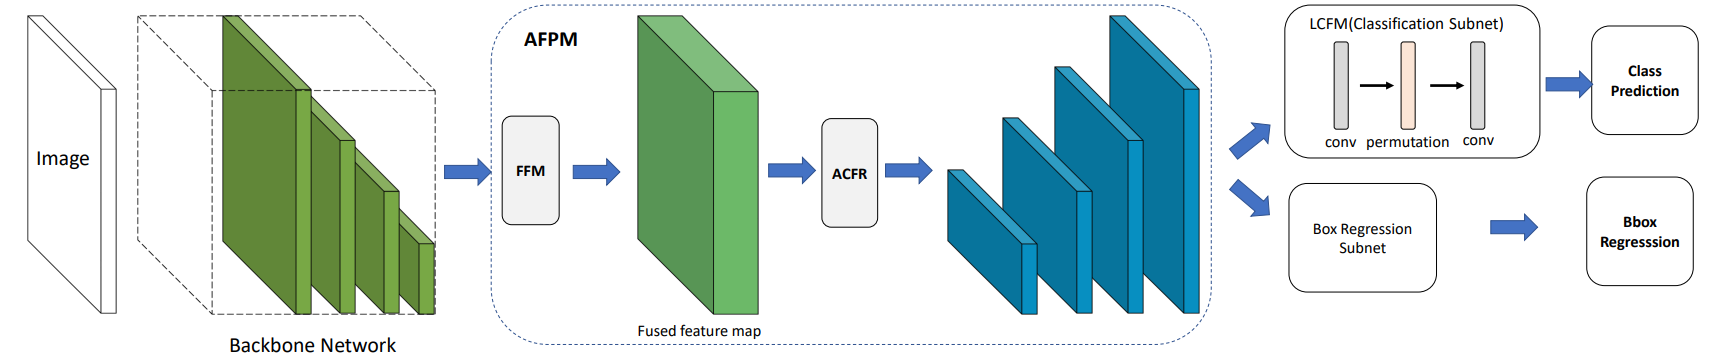
\includegraphics[width=0.9\textwidth]{Figures/LADet.PNG} 
        \caption{An overview of LADet model. Multi-level feature maps from the backbone network are processed by the \gls{afpm} to create pyramid feature maps. These enhanced maps are then used by the \gls{lcfm} and the box regression subnet to generate classification scores and dense bounding boxes.\cite{LADet}.}
        \label{LADet}
    \end{figure}

     Experiments demonstrate LADet's effectiveness on PASCAL VOC and MS COCO datasets. It achieves a \gls{map} of 81.4\% on PASCAL VOC and an average precision of 33.6\% on MS COCO at 20.8 \gls{fps}. This performance strikes an impressive balance between accuracy and efficiency, making LADet a strong candidate for real-time \gls{od} tasks \cite{LADet}.
     
\end{enumerate}

\section{Selection Criteria of Camera Systems}
Choosing the right \gls{cs} is a very important milestone in every computer vision project. An unsuitable system can complicate \gls{sw} requirements, as it may require extensive pre-processing, lead to lost or degraded image assets, and in many cases can result in project failure. In order to avoid that, one should carefully follow a systematic approach in choosing a CS. This process requires a careful evaluation of key features to ensure that the hardware is optimally aligned with the project’s specific objectives.

Key technical considerations in CS selection include the scanning method, resolution, \gls{dr}, sensor size, frame rate, shutter type, and \gls{fov}. Additional factors, such as lens type, communication protocol, mounting techniques, environmental conditions, and budget requirements, should also be evaluated to improve the robustness of the system and its compatibility with the demands of the project.

\subsection{Scanning Method}
The camera's scanning or imaging method is a primary factor in determining the appropriate camera type for a given application. The most commonly used scanning methods are line scan and area scan.

\subsubsection{Line Scan Cameras}
Line scan cameras operate with a single row of pixels arranged on a long, narrow sensor. As the target object moves along the narrow axis of the sensor, the camera captures data one row of pixels at a time, constructing the complete image through sequential \gls{sw} processing. This method requires careful synchronization between the sensor scan time and the movement of the object to produce a stable and accurate image output. The continuous image-building capability makes line scan cameras particularly well suited for high-speed applications such as print inspection and document scanning, where maintaining image quality over fast moving objects is critical \cite{AS_VS_LS_ART}.

A primary advantage of line scan cameras is their ability to capture continuous images without being limited by a fixed vertical resolution, resulting in significantly higher resolution than area scan cameras. Additionally, these cameras are optimized for high-speed processing environments, as they enable rapid image acquisition and efficient data transfer. Since the pixel readout rate is faster than the exposure time, line scan cameras can initiate a new capture while the previous image is still transferring, maximizing their efficiency in fast-paced settings. This feature makes them ideal for applications that demand rapid, uninterrupted image acquisition \cite{AS_VS_LS_ART}.

However, line scan cameras also come with limitations. The need for precise synchronization between the sensor’s capture timing and the moving object’s speed is crucial to maintaining image stability, which can be challenging to achieve in dynamic environments. Furthermore, line scan cameras are limited in their ability to capture static images or video of moving objects, as they rely on the movement of the object to construct the image. The installation process is often complex and costly, requiring specialized setups that can increase the overall expense of a project. Despite these limitations, line scan cameras remain invaluable in high-resolution, high-speed applications where traditional imaging methods may fall short \cite{AS_VS_LS_ART}.

\subsubsection{Area Scan Cameras}
On the other hand, area scan cameras have a matrix of pixels that captures the data of the image in a single exposure. The camera structure of an area scan camera typically consist of an array sensor, such as a charge coupled device or complementary metal oxide semiconductor known as CMOS, where each pixel represents part of the entire image captured in a single exposure \cite{AS_VS_LS_ART}. 

Area scan cameras are more cost-effective choice since they are simpler to use and easier to install than line scan cameras. Their versatility extends to tasks requiring strobe lighting for moving objects and allows for real-time video display on monitors, a feature which is very much appreciated when real time video processing is required. Unlike line scan cameras, which must capture multiple rows of data to assemble a full image, area scan cameras can capture a defined area in a single exposure which results in saving time and simplifying the imaging process. Additionally, area scan cameras offer the flexibility to divide a single image into multiple regions of interest to allow specific \gls{od} within different areas of the frame simultaneously. However, it still comes with the limitation in its \gls{fov}, unlike the line scan camera, which has a wide \gls{fov}, the area scan camera is restricted in this aspect. Figure~\ref{AS_VS_LS_PIC} illustrates a comparison between area scan and line scan cameras in terms of their working principles.

\begin{figure}[h]
    \centering
    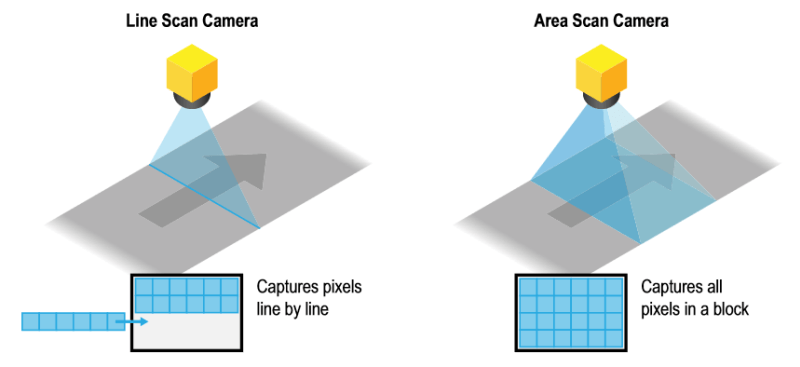
\includegraphics[width=0.7\textwidth]{Figures/Line-Scan-v-Area-Scan.png}  
    \caption{Comparison of area scan and line scan cameras \cite{AS_VS_LS_PIC}.}
    \label{AS_VS_LS_PIC}
\end{figure}


\subsection{Resolution}
Camera resolution is a key parameter to be considered when working with \gls{dl} projects. It refers to the number of pixels used to represent an image. Image resolution directly influences the quality of data input into a \gls{dl} model. Higher resolution images provide more detailed information, which can improve the model's performance for tasks such as \gls{od}, image segmentation, and classification. For example, in medical imaging or satellite data analysis, higher resolution can capture fine details that are important for diagnosis or analysis. However, as the resolution increases, so does the computational cost in terms of memory and processing time, making it important to find a balance between image quality and efficiency.

Several studies have investigated the impact of image resolution on \gls{cnn} performance across various fields, including medical imaging. For instance, Thambawita et al. \cite{RES_IMP} conducted an experimental study using the HyperKvasir dataset, which consists of 10,662 endoscopic images covering 23 different gastrointestinal conditions. Their research focused on how changes in image resolution influence \gls{cnn} performance,  particularly in the context of endoscopic image classification. The study focused on image resolutions ranging from 32×32 to 512×512 pixels and evaluated the performance of two \gls{cnn} architectures: ResNet-152 and DenseNet-161. Figure~\ref{RES_COMP} shows the differences in image quality for different image resolutions. 
\begin{figure}[ht]
    \centering
    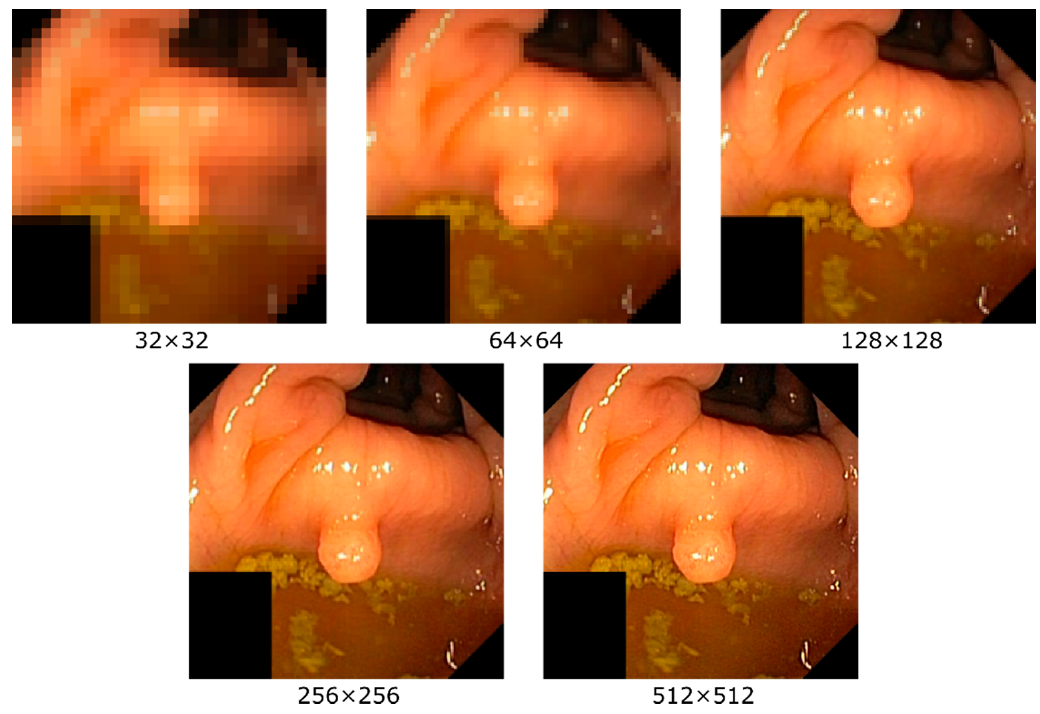
\includegraphics[width=0.7\textwidth]{Figures/RES_COMP.png}  
    \caption{Example of images that were used in the study to show the differences in level of details that are observed from different resolutions. Note that for this figure all pictures are rescaled to the same size to show quality differences \cite{RES_IMP}.}
    \label{RES_COMP}
\end{figure}

The study \cite{RES_IMP} found that higher resolution images consistently led to improved classification accuracy and precision. Specifically, the use of 512×512 pixel images resulted in the highest performance metrics, with a Matthews Correlation Coefficient (MCC) of 0.9002. The research highlighted that high-resolution images better preserved fine details, such as surface textures and subtle features of lesions, which are essential for accurate classification in medical contexts. On the other hand, lowering the resolution caused a notable decline in performance, particularly in detecting subtle abnormalities like Barrett’s esophagus.

It was also highlighted in a study by Barkat et al. \cite{RES_HDR_IMP}, capturing images at 42 MP resolution, combined with \gls{hdr} techniques, significantly improves the clarity of visual data, especially in low-light conditions. This improvement enables more accurate detection and classification of events like avalanches using \gls{dl} algorithms. Furthermore, the high-resolution images provide detailed information that allows for the identification of subtle surface deformations, which are essential for detecting early signs of avalanches. The study highlights that such critical details would be missed with lower resolution images, stressing the importance of maintaining high resolution in optical monitoring systems to ensure both accuracy and reliability in \gls{dl}-based detection.

One of the primary challenges highlighted in the study by Thambawita et al. \cite{RES_IMP} was the significant increase in computational cost associated with processing higher-resolution images. The use of larger images in the training of \gls{cnn} requires more memory and processing power. As a result, it becomes necessary to reduce the batch size to fit these higher-resolution images within the limited capacity of the available GPU memory. Even with the extra computational demands, the research showed that using higher-resolution images led to better performance, which made the trade-offs worthwhile.

In the context of \gls{dl}-based text and object recognition for motorbike \gls{db}s, similar findings can be drawn from the studies. For example, a key issue is recognizing text with low contrast against the background or in small fonts, making it difficult for standard recognition systems. Using higher resolution camera images can improve clarity, allowing models to better detect and process this information. However, this solution must be balanced with the computational power required, as higher resolution images demand more resources. To ensure feasibility in practical applications, it is important to optimize both accuracy and processing efficiency in these systems.

\subsection{Dynamic Range}
\gls{dr}  is defined as the ratio between the highest and lowest light intensities a system can handle without losing information. In digital imaging, this range often reflects how well a camera can adapt to bright and dim elements in the same scene. Mukherjee et al. describe \gls{hdr} as an advanced imaging technique designed to capture and process a wide spectrum of visible lighting conditions, \gls{hdr} imaging encompasses a broad range of luminance values, spanning approximately 13 orders of magnitude, from \( 10^{-4} \) to \( 10^8 \ \text{cd/m}^2 \) \cite{HDR}. Direct sunlight can have luminance values up to approximately \( 1.6 \times 10^9 \, \text{cd/m}^2 \) \cite{sunlight_lum}.This large range of brightness levels is why \gls{hdr} is used to capture both very dark and very bright areas in a scene accurately. To capture and represent this range, \gls{hdr} scene information is often stored in high precision formats, using 32 or 16 bits per pixel per channel, in file types like \texttt{.hdr} or \texttt{.exr}. floating point formats. This range is closely aligned with the human eye’s ability to perceive various light levels. In contrast, \gls{sdr} imaging compresses scene details into a more limited range, around 3 orders of magnitude, which can restrict visibility in extreme lighting. \gls{hdr}, on the other hand, captures luminance from very dark shadows to intensely bright highlights, preserving critical details essential for precise \gls{od} in complex lighting environments \cite{HDR}.

\gls{dr} is considered one of the most vital parameters when choosing a \gls{cs} for \gls{dl} purposes especially in the field of \gls{od}. Various studies discussed the impact of \gls{dr} on detecting objects in challenging lighting conditions. for instance, Mukherjee et al. presented a method to develop an \gls{hdr} dataset from existing \gls{sdr} datasets to train models without needing \gls{hdr}-specific image libraries. Their approach involves using \gls{cnn}-based expansion operators to convert \gls{sdr} images into \gls{hdr} format. They then test \gls{od} models, specifically Faster \gls{rcnn} and \gls{ssd}, on both \gls{hdr} and \gls{sdr} datasets. To further evaluate model performance in realistic settings, they included an out of distribution \gls{hdr} dataset created with native \gls{hdr} cameras. Their findings reveal that models trained on \gls{hdr} data perform 10–12\% better in accuracy than those trained on \gls{sdr} data, particularly in high-contrast scenes, demonstrating superior \gls{od} in complex lighting conditions \cite{HDR}. Figure~\ref{fig:HDR vs SDR} showes the comparison presented in the study between \gls{hdr} detection (Figure~\ref{HDR}) and \gls{sdr} Detection (Figure~\ref{SDR}). It is clear that \gls{hdr} trained detectors successfully detected all assets of the picture, while \gls{sdr} failed to detect 4 of the assets.

\begin{figure}[ht]
    \centering
    % First subfigure
    \begin{subfigure}[b]{0.45\textwidth}
        \centering
        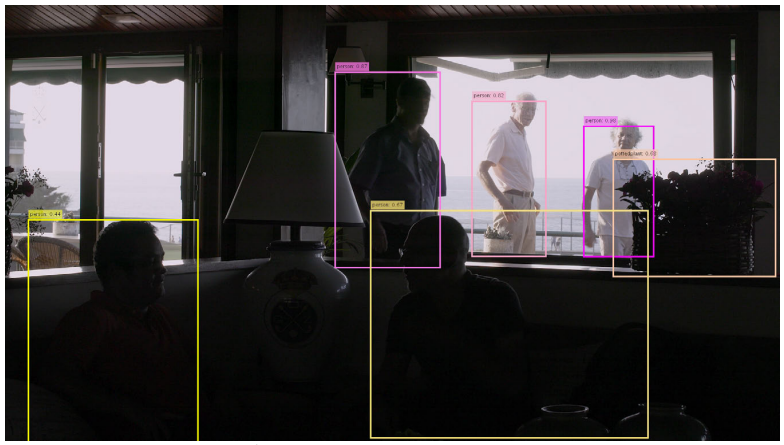
\includegraphics[width=\textwidth]{Figures/HDR.PNG}
        \caption{\gls{hdr} Detection}
        \label{HDR}
    \end{subfigure}
    \hfill
    % Second subfigure
    \begin{subfigure}[b]{0.45\textwidth}
        \centering
        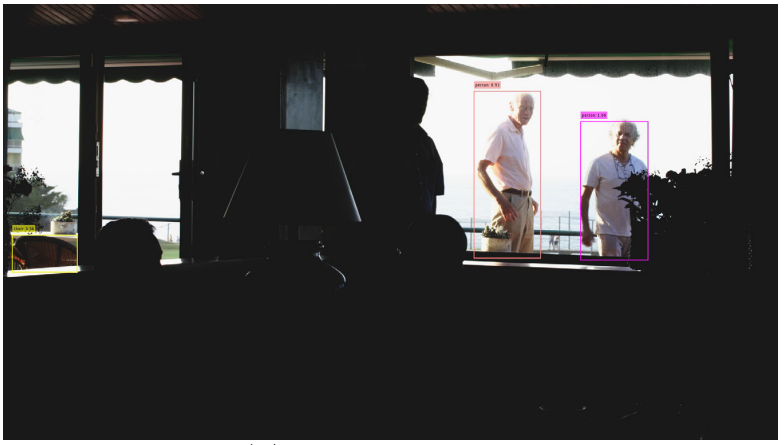
\includegraphics[width=\textwidth]{Figures/SDR.PNG}
        \caption{\gls{sdr} Detection}
        \label{SDR}
    \end{subfigure}
    
    \caption{Example image showing the comparison results between \gls{hdr} and \gls{sdr} detection \cite{HDR}.}
    \label{fig:HDR vs SDR}
\end{figure}

Using \gls{hdr} imaging in \gls{dl} offers several benefits, such as improved model accuracy and stronger resilience to varying real-world lighting challenges. \gls{hdr} provides richer visual information, allowing models to train on a wider range of lighting conditions, which enhances their ability to generalize and reduces the likelihood of errors in unfamiliar settings. This makes \gls{hdr} valuable in applications where accuracy and reliability are important. However, \gls{hdr} also brings certain challenges. The higher bit-depth and extended range of \gls{hdr} images demand more storage and computational power for both training and inference, which can lead to longer processing times and higher costs during deployment.

To overcome such limitations, one can use Tone Mapping Operators to map the \gls{hdr} content to \gls{sdr} content without loosing the assets in the original scene, this is done using a tone-compression curve, it works by changing the 16/32 bit floating point to 8 bit channels such that the resultant pixel value is ranging between 0 to 255 \cite{HDR}.

\subsection{Sensor Size}
The term sensor size in \gls{cs}s refers to the physical dimensions of the imaging sensor, which captures light and converts it into electrical signals to create digital images. Figure~\ref{Sen_Size_chart} Shows how sensor size changes between multiple devices. Generally, larger sensors are able to capture more light, resulting in images with more detail, less noise, and enhanced \gls{dr}. Recent research highlights the importance of sensor size in determining image quality, especially in low-light settings or high-contrast scenes. This makes sensor size a critical factor in applications such as \gls{od}, image classification, and scene recognition within \gls{dl}, where high-quality images can significantly impact model performance.
\vspace{0.5 cm}
\begin{figure}[ht]
    \centering
    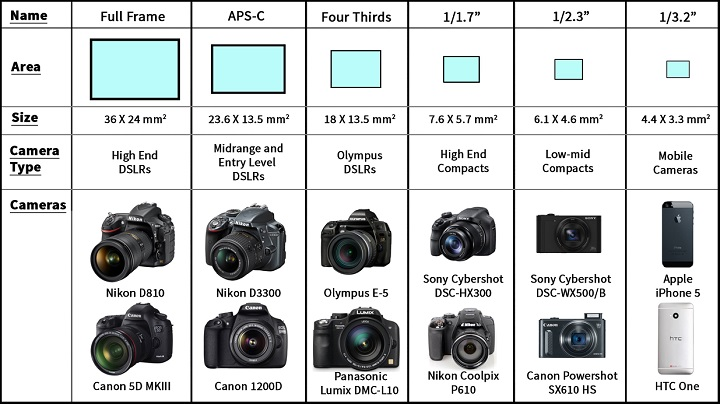
\includegraphics[width=0.8\textwidth]{Figures/sensor-chart.jpg}  
    \caption{Use case of different sensor sizes and their used application \cite{Sen_size_chart}.}
    \label{Sen_Size_chart}
\end{figure}

Another crucial factor to consider when selecting a sensor size is the required resolution, as resolution and sensor size are closely related. In simple terms, resolution refers to the number of pixels in an image as explained earlier. If the sensor is small but the resolution requirement is high, each pixel will occupy only a tiny space on the sensor, receiving minimal light. This limited light per pixel generally leads to lower image quality and increased noise. Conversely, with a larger sensor, each pixel has more room and can capture a greater share of light, which enhances overall image quality by reducing noise and improving detail.

In a study \cite{Sensor_size} investigates how specific camera parameters, including sensor pixel size, influence the generalization of \gls{cnn}s in \gls{od} tasks. The authors used synthetic data generated with the ISETAuto soft prototyping tool, which simulates camera images under various conditions to control parameters like pixel size, bit-depth, and exposure. In this experiment, the effect of changing sensor's characteristics on \gls{cnn} ability to generalize across datasets was evaluated, including synthetic and real-world images. The study found that pixel size significantly impacts model performance, especially in generalization across varied environments. One can directly relate pixel size with sensor size because it is the amount of physical dimension required per pixel, and that is directly proportion to the size of the sensor for a given resolution.

In terms of methodology, The authors created synthetic images with varying pixel sizes (from 1.5 µm to 6 µm) and trained a \gls{cnn} on these images. They then evaluated the model’s ability to generalize to other datasets, including KITTI, BDD, and CityScape, which are standard datasets in autonomous driving research. The results demonstrated that smaller pixel sizes generally led to better generalization performance, likely due to the higher spatial resolution afforded by smaller pixels, which allows the model to capture finer details essential for \gls{od}. However, as pixel size increased, the model’s ability to generalize decreased, resulting in poorer performance on datasets with varying lighting and scene conditions.

This study illustrates the critical role of sensor size (specifically pixel size) in determining the quality of data for \gls{dl} applications. Smaller pixel sizes, associated with higher spatial resolution, enable \gls{cnn}s to learn more detailed features, which is essential for tasks requiring precision, such as \gls{od} in varying environments. However, larger pixel sizes, while potentially more light-sensitive, may reduce resolution and, consequently, model performance in diverse scenes. These findings suggest that optimizing sensor size for specific \gls{dl} tasks is essential, as it directly impacts the accuracy, robustness, and generalization capabilities of \gls{ai} models, particularly in complex real-world environments like autonomous driving.

\subsection{Frame Rate}

Frame rate, expressed in \gls{fps}, plays a crucial role in the performance of \gls{od} models in computer vision. Higher frame rates can provide more frequent image updates, enabling the system to detect fast-moving objects with greater precision and maintain smoother visual tracking. This allows for improved responsiveness and accuracy in dynamic environments. In a study to optimize \gls{od} in autonomous vehicles using gray scale computer vision models \cite{FPS}, the authors argued that increasing frame rate enhances \gls{od} accuracy by providing higher temporal resolution, particularly in dynamic environments like autonomous vehicle navigation.

The authors claimed that high frame rates play a crucial role in real-time \gls{od} by proving that it  minimizes the distance a vehicle travels between captured frames, therefor enhancing decision-making speed. For example, at a velocity of 80 km/h, a camera operating at 60 \gls{fps} corresponds to 37 cm of travel per frame. Doubling the frame rate to 120 \gls{fps} reduces this distance to 18.5 cm per frame, allowing earlier and more accurate detection and response to objects. This improvement is particularly significant in high-speed and complex scenarios where timely and precise decisions are needed. Moreover, higher frame rates improve the detection of fast-moving or distant objects by providing a more continuous and detailed input stream for the detection model.

In an application such as \gls{db} testing where objects and texts are stationary for the current generation, it's not necessary to consider such a parameter when choosing a CS. However, it is expected to have high more animations and graphics in the future generations of \gls{db}, that is why it could be a good investment to include such a parameter in the decision making process if the resources allow.


